\documentclass[10pt,a4paper]{beamer}

\usepackage[utf8]{inputenc}
\usepackage[russian]{babel}
\usepackage[OT1]{fontenc}
\usepackage{amsmath}
\usepackage{amsfonts}
\usepackage{amssymb}
\usepackage{makeidx}
\usepackage{graphicx}
\usepackage{xcolor}
\usepackage{multirow}
\usepackage{framed}
\definecolor{shadecolor}{cmyk}{0,0,0,1}
\usepackage{hyperref}
\usepackage[normalem]{ulem}

\titlegraphic{
   
\includegraphics[width=4cm]{images/sfera.jpg}
}

\author{Николай Анохин \and Михаил Фирулик}
\title{Введение в Data Science \\ Занятие 13. Заключительное}

\beamertemplatenavigationsymbolsempty

\begin{document}

\maketitle

\logo{
    
\includegraphics[width=4cm,keepaspectratio]{images/sfera.jpg}\hspace{0.45em}
}

\begin{frame}

\tableofcontents

\end{frame}

% ============================================== %

\section{Предобработка данных}

% ============================================== %

\begin{frame}{Выбор параметров модели}

\begin{center}
\hspace{-3em}
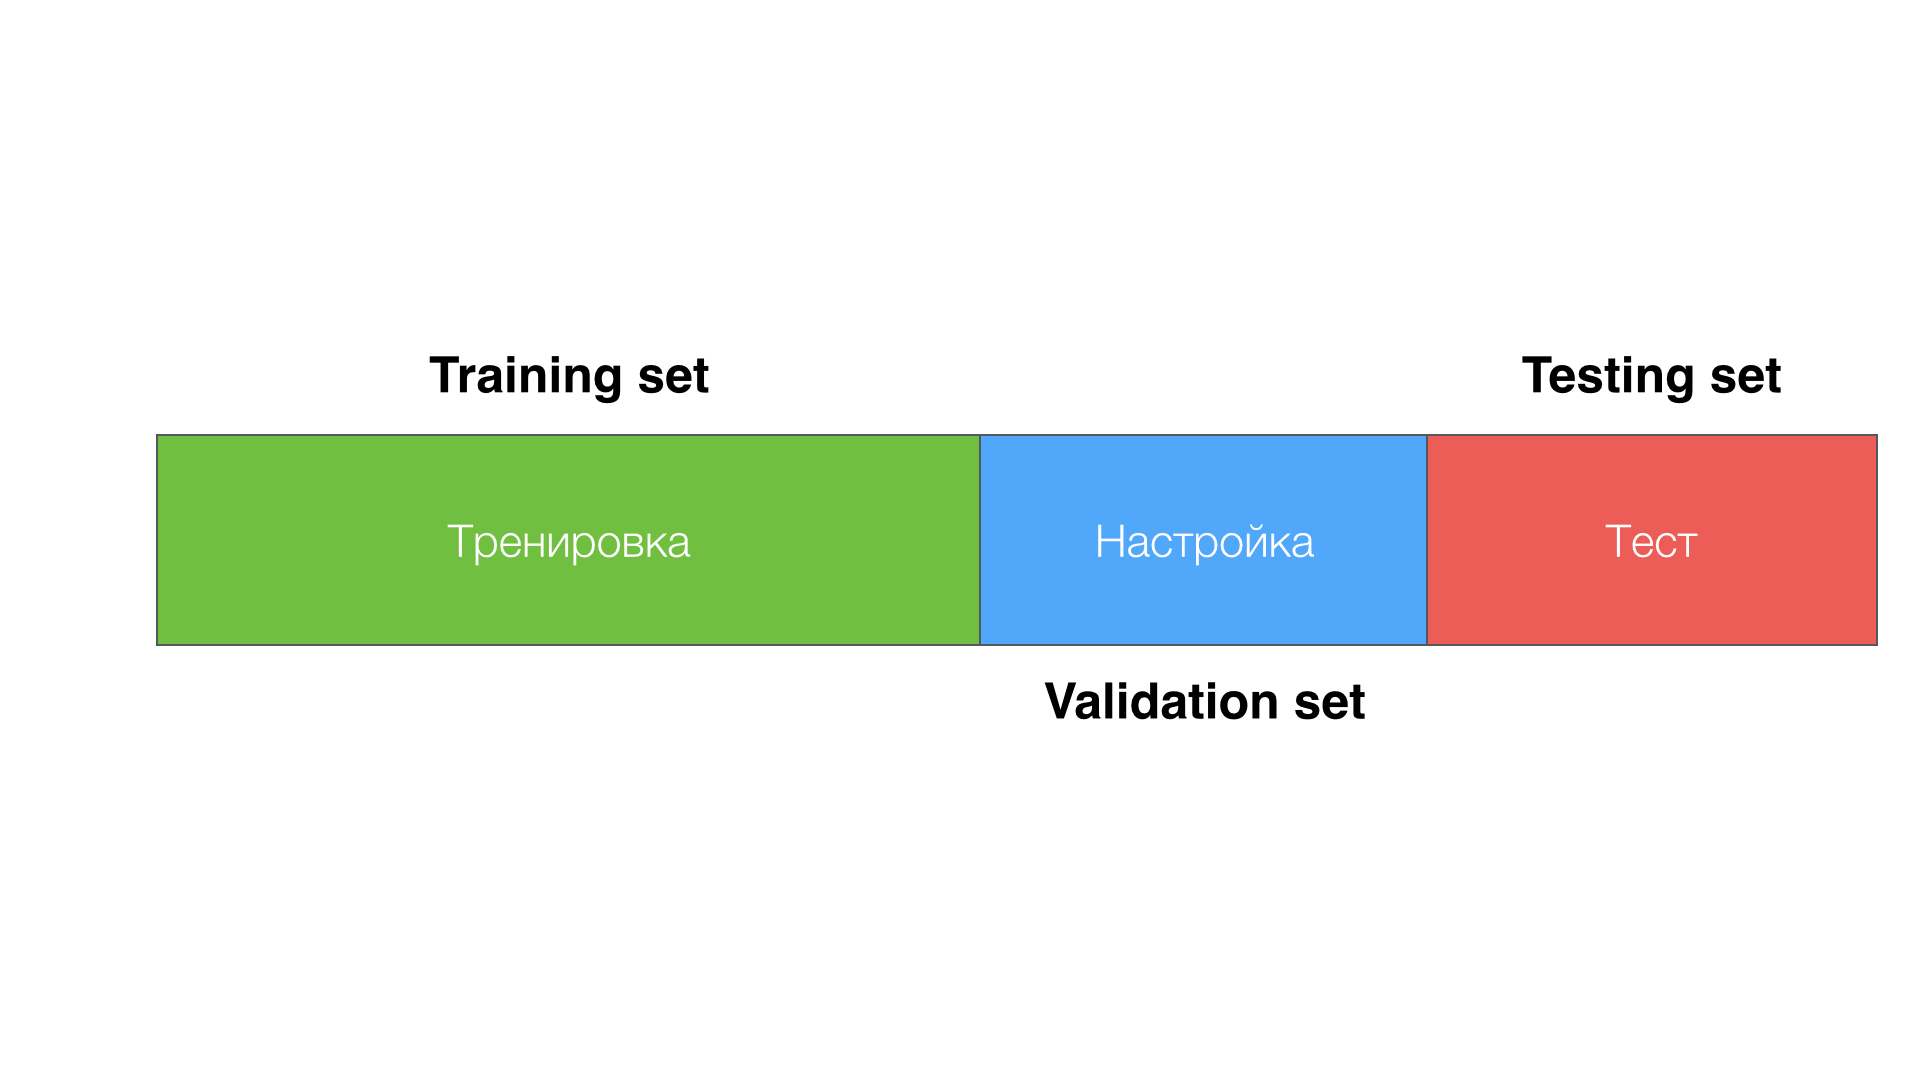
\includegraphics[scale=0.15]{images/vtt.png}
\end{center}

\end{frame}

% ============================================== %

\begin{frame}{Предобработка данных}

\begin{itemize}
\item {\bf выбор признаков} / feature selection
\item дискретизация признаков / feature discretization
\item очистка данных / data cleansing
\item уменьшение размерности / dimensionality reduction
\end{itemize}

\end{frame}

% ============================================== %

\begin{frame}{Зачем выбирать признаки?}

\begin{center}
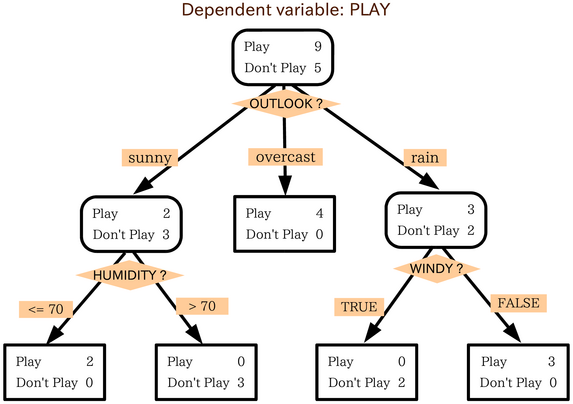
\includegraphics[scale=0.3]{images/dt.png}
\end{center}

\begin{enumerate}
\item Качество \\
{\it подвержены влиянию случайных признаков: DT, KNN, ...}
\item Скорость \\
{\it хотя отбор признаков на практике медленный}
\item Интерпретируемость
\end{enumerate}

\end{frame}

% ============================================== %

\begin{frame}{Подходы к выбору признаков}

\begin{itemize}
\item Ручной \\
{\it лучше, если вы знаете, что делаете}
\item Автоматизированный \\
\begin{itemize}
\item Схемо-независимый / Scheme-independent
\item Схемо-зависимый / Scheme-specific
\end{itemize}
\end{itemize}

\end{frame}

% ============================================== %

\begin{frame}{Схемо-независимый подход}

\begin{columns}[T]
    \begin{column}{.5\textwidth} 
	\begin{itemize}
	\item Выбрать столько, чтобы идентифицировать каждый объект
	\item Техника near-hit, near-miss
	\item С помощью выбранного критерия качества
	\item С помощью алгоритма машинного обучения \\
	{\it Decision Tree, Linear Model}	
	\end{itemize}
    \end{column}
    \begin{column}{.5\textwidth} 
	\begin{center}
	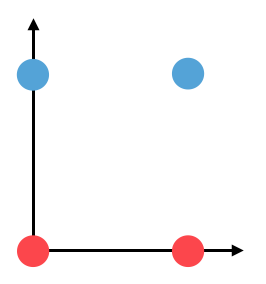
\includegraphics[scale=0.3]{images/hit-miss.png}
	\end{center}  
    \end{column}
\end{columns}

\end{frame}

% ============================================== %

\begin{frame}{Критерии качества признаков}

{\bf Сколько?}
\begin{itemize}
\item Фиксированное количество \\
{\it Пример: лучшие 100 признаков}
\item Percentile \\
{\it Пример: лучшие 20 процентов}
\end{itemize}

{\bf Как?}
\begin{itemize}
\item Mutual Information
\[
I(X, Y) = \sum_x \sum_y p(x, y) \log \left( \frac{p(x, y)}{p(x) p(y)} \right)
\]
\item Statistical Tests \\
{\it $Chi^2$, $binomial$, ...}
\end{itemize}

\end{frame}

% ============================================== %

\begin{frame}{Схемо-зависимый поиск в пространстве признаков}

\begin{center}
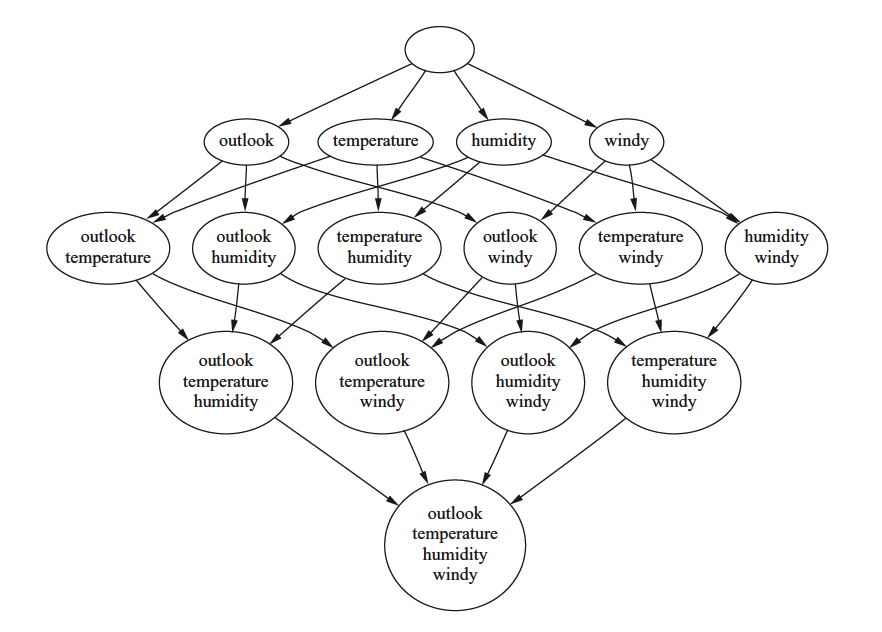
\includegraphics[scale=0.25]{images/lattice.png}
\end{center}

\begin{itemize}
\item Forward-selection
\item Backward-elimination
\end{itemize}

\end{frame}

% ============================================== %

\section{Заключение}

% ============================================== %

\begin{frame}{Что мы рассмотрели: классификация}

\begin{center}
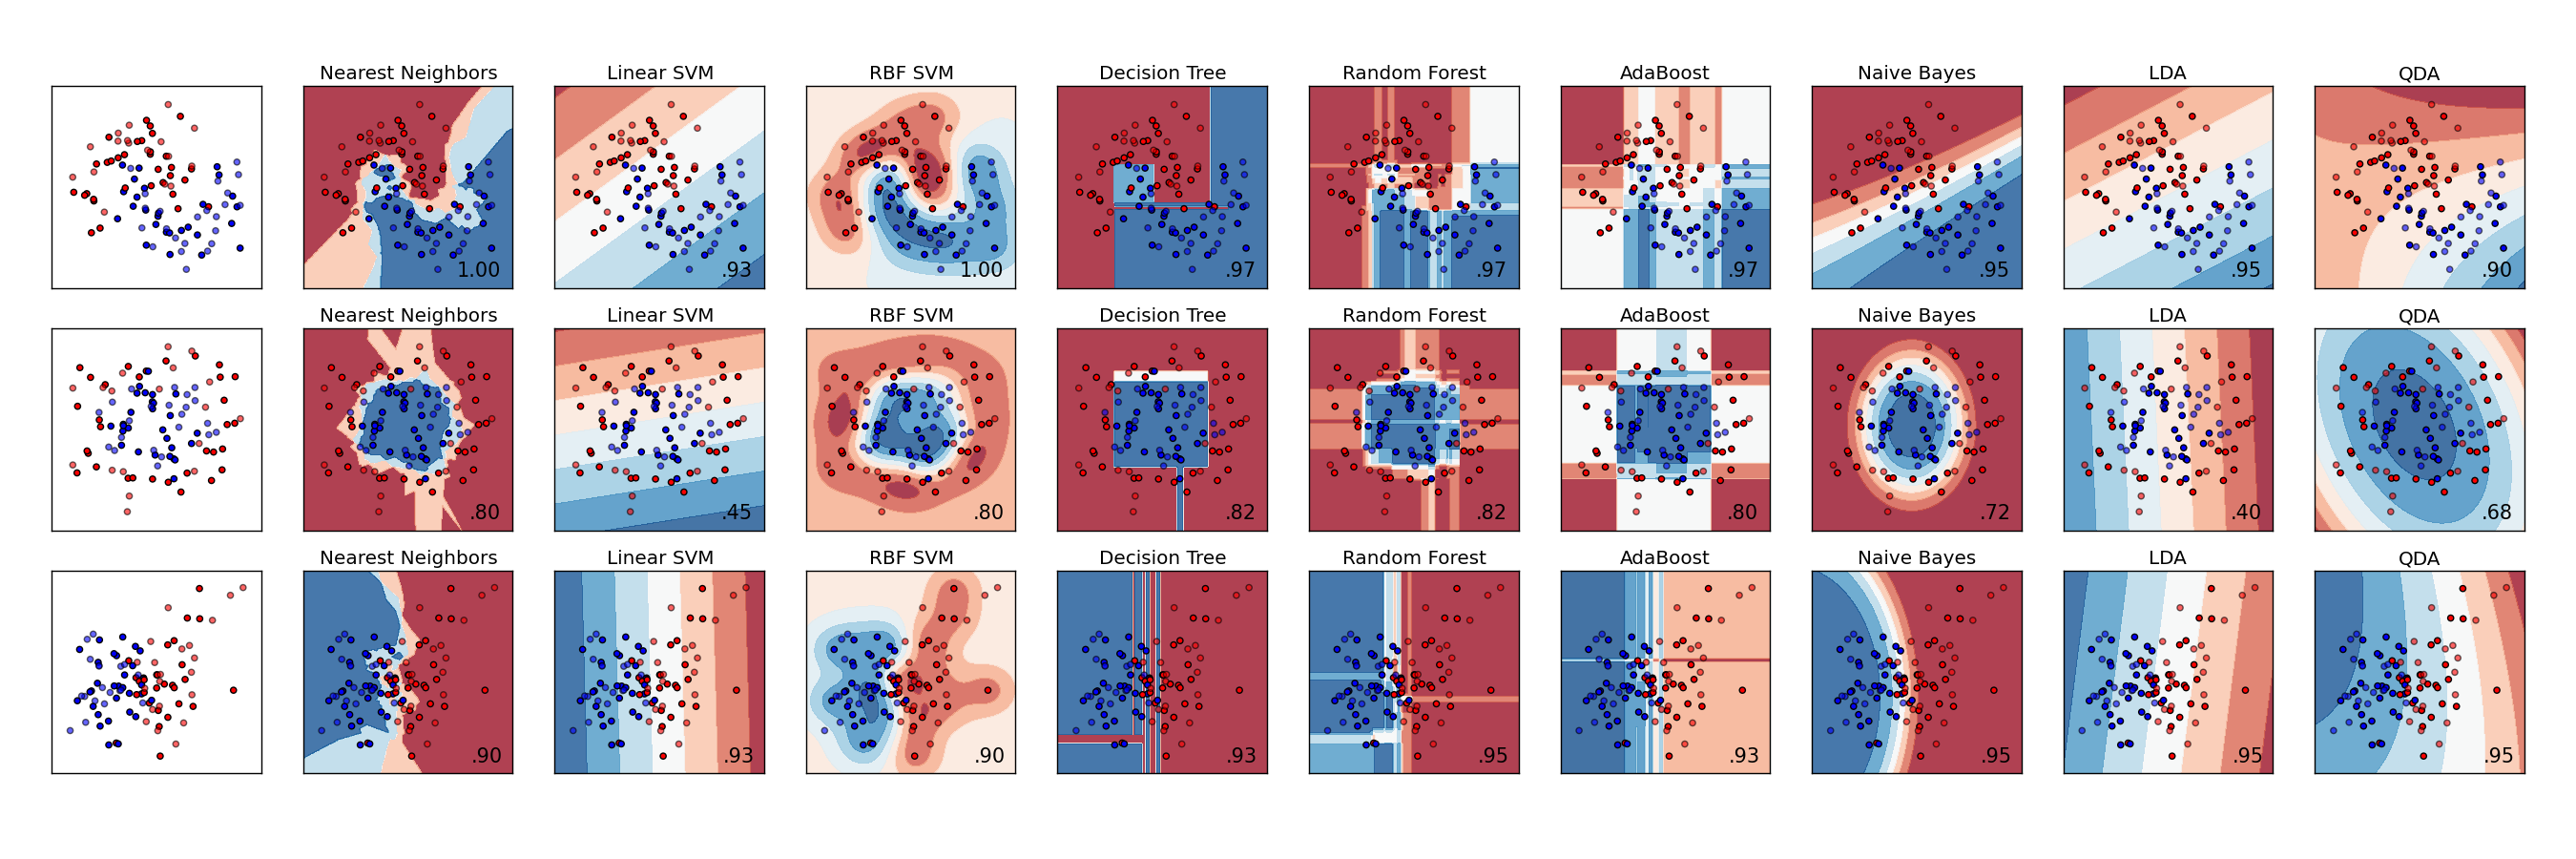
\includegraphics[scale=0.16]{images/classification.png}
\end{center}

\end{frame}

% ============================================== %

\begin{frame}{Что мы рассмотрели: кластеризация}

\begin{center}
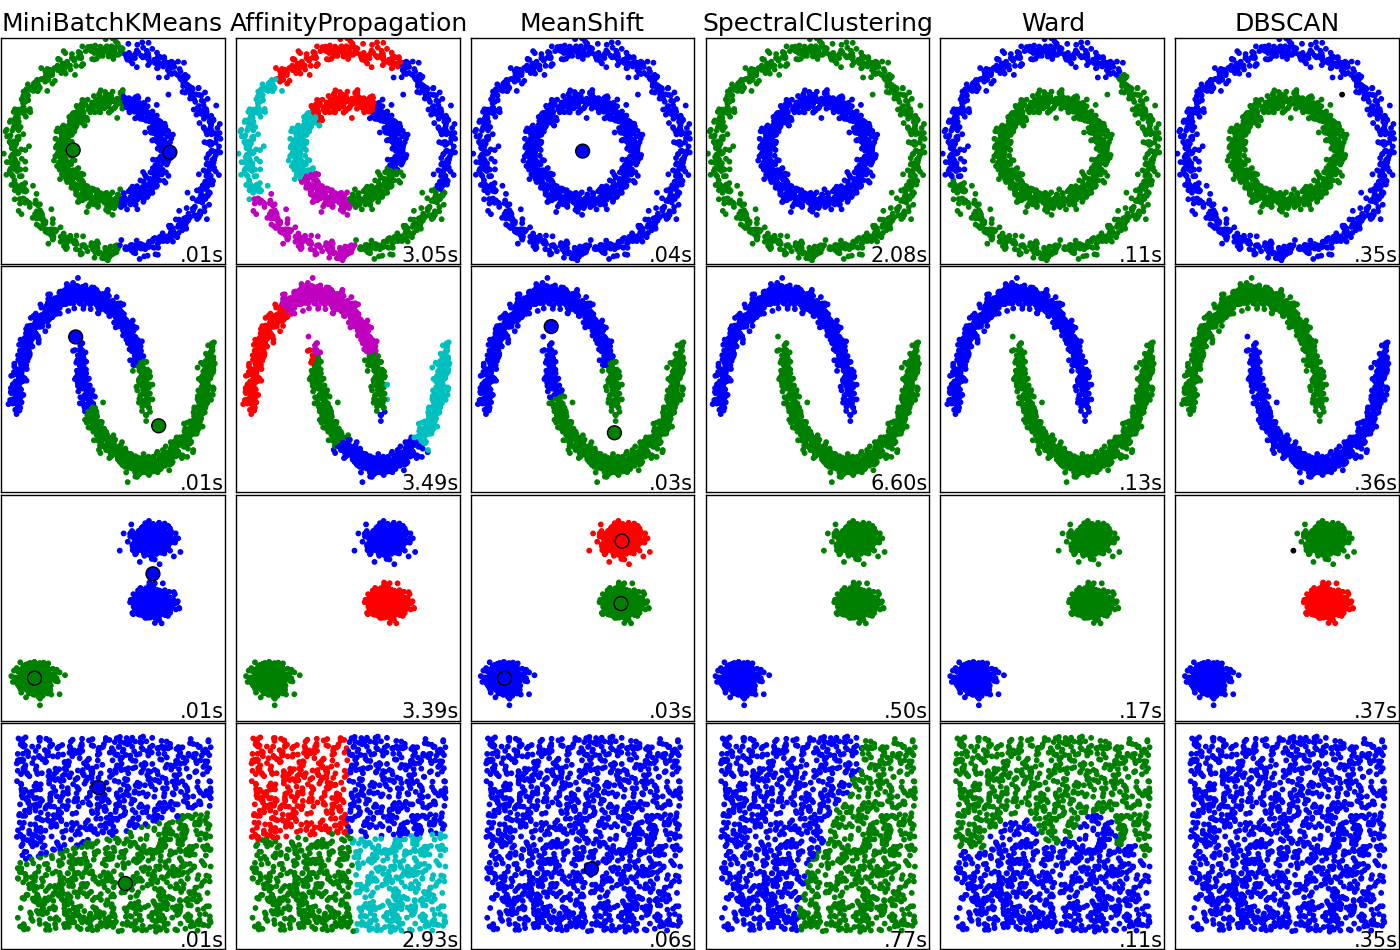
\includegraphics[scale=0.2]{images/clustering.png}
\end{center}

\end{frame}

% ============================================== %

\begin{frame}{Что мы рассмотрели: технологии}

\begin{center}

\includegraphics[scale=0.3]{images/scipy.png} \quad \quad \quad

\includegraphics[scale=0.8]{images/sklearn.png}


\includegraphics[scale=0.3]{images/hadoop.jpg}
\end{center}

\end{frame}

% ============================================== %

\begin{frame}{Что мы не рассмотрели}

\begin{columns}[C]
    \begin{column}{.4\textwidth}
    \begin{itemize}
	\item neural networks
	\item genetic algorithms
	\item dimensionality reduction
	\item semi-supervised learning
	\item reinforcement learning
	\item NLP, SNA
	\item и еще много чего
	\end{itemize}
    \end{column}
    \begin{column}{.6\textwidth} 
	\begin{center}
	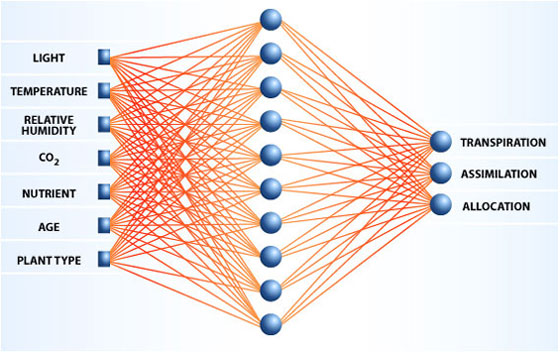
\includegraphics[scale=0.3]{images/nn.jpg}
	\end{center}  
    \end{column}
\end{columns}

\end{frame}

% ============================================== %

\begin{frame}{Что делать дальше}

\begin{itemize}
\item Kaggle \url{http://blog.kaggle.com/}
\item Hilary Mason \url{http://www.hilarymason.com/}
\item Alex Holmes \url{http://grepalex.com/}
\item Cloudera \url{http://blog.cloudera.com/}
\item Coursera
\item Аспирантура (+PhD)
\item Трудоустройство
\item Собственный проект
\end{itemize}

\end{frame}

% ============================================== %

\begin{frame}{}

\begin{center}
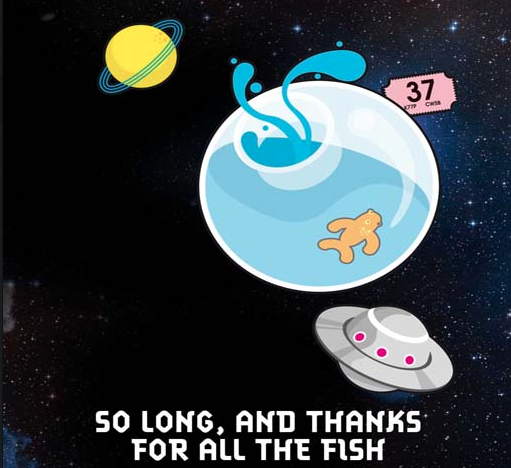
\includegraphics[scale=0.43]{images/fish.png}

m.firulik$@$corp.mail.ru \quad n.anokhin$@$corp.mail.ru

\end{center}

\end{frame}

% ============================================== %

\begin{frame}{На самом деле, еще не совсем все}

\begin{columns}[C]
    \begin{column}{.5\textwidth}
    Результаты (17 июня 00.00)
	\begin{itemize}
	\item Код на bb
	\item Проклассифицированные пользователи
	\end{itemize}
	Презентация (17 июня 09.30)
	\begin{itemize}
	\item Использованные признаки
	\item Выбранная модель
	\item Результаты классификации
	\end{itemize}
	Время: 10 + 5 мин
    \end{column}
    \begin{column}{.5\textwidth} 
	\begin{center}
	
\includegraphics[scale=0.25]{images/doge.jpg}
	\end{center}  
    \end{column}
\end{columns}

\end{frame}

\end{document}